\section{Desenvolvimento}
	Nesta seção, vamos mostrar e explicar os artefatos utilizados no processo de 
	design (produção) da interface a partir dos modelos de interação.
	\subsection{Da Interação Para o Design}
		Para poder realizar o design de interface para um sistema computacional, é necessário que hajam cenários 
		de interação nos quais se basear. Isto é, não se pode produzir uma interface 
		sem que se saiba de antemão os objetivos e funções que o sistema deverá oferecer.
		
		Por esse motivo, nosso trabalho foi baseado em Modelos de Mnteração, os 
		quais por sua vez são baseados em Cenários de Interação. Cenários de Interação 
		são descrições brevemente detalhadas sobre as ações do usuário e as respectivas
		respostas do sistema necessárias para o usuário alcançar seus objetivos \cite{ihc:barsil}. 
		Modelos de Interação são baseados em cenários de interação, e são constituídos 
		pelas conversas que o usuário vai ter com o sistema durante sua utilização.
		
		A modelagem que seguimos foi a que está disponível em \cite{ihc:barsil}. Ela 
		é formulada na linguagem de modelagem MoLIC\footnote{Modeling Language for Interacion 
		as Conversation}. MoLiC é uma linguagem para a modelagem da interação humano-computador
		como uma conversa, que as constrói em formato de diagramas de fluxo. A 
		elaboração de modelos dessa ordem é um passo anterior 
		ao design de interface, assim por esse motivo não estaremos explicando como 
		são elaborados tais modelos.
		
		O diagrama MoLIC em que o design foi baseado é um modelo de sistema de apoio 
		ao professor, sendo que este deverá poder lançar avisos aos alunos, disponibilizar 
		materiais e avaliar atividades enviadas pelos alunos. A figura seguinte ilustra 
		o próprio diagrama:
		
		\begin{figure}[!ht]
			\centering
			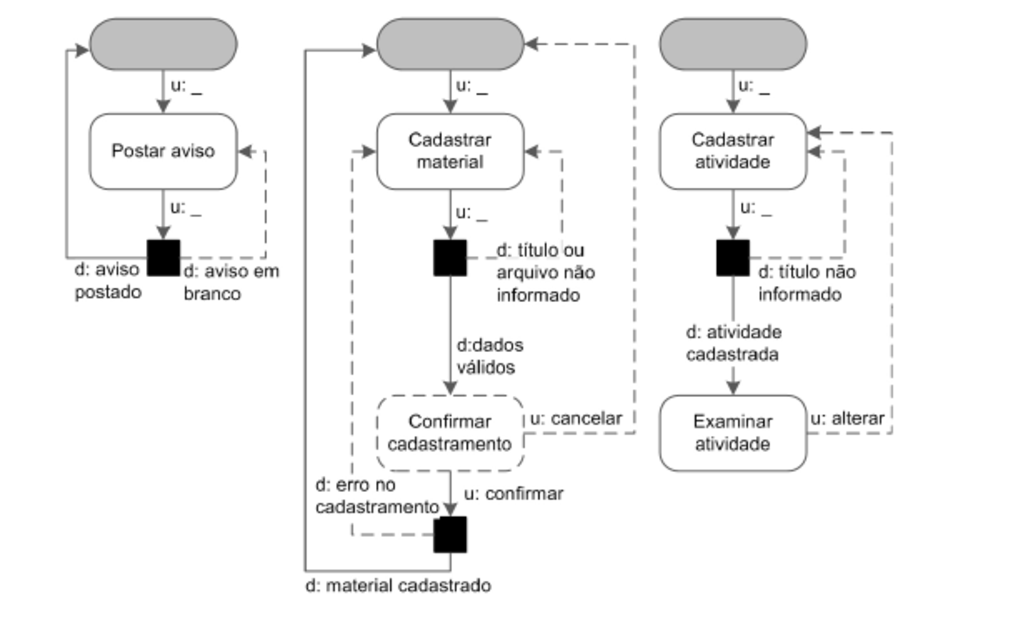
\includegraphics[scale=0.7]{molic.pdf}
			\caption{Diagrama MoLIC em que a interface foi baseada}
		\end{figure}
		
	\subsection{Design de Interface}
	
		\subsubsection{Estilos de Interação}
A definição da interface inicia com a escolha do estilo de interação do sistema
para então passar a representação da interface.	Os estilos de interação mais
comuns são linguagens de comando, linguagem natural e a interação por menus,
formulários, manipulação direta e WIMP (Windows, Icons, Menus and Pointers).


	Em uma interação por linguagem de comando, o usuário interage com o sistema
por comandos digitados, os quais realizam ações na aplicação. Para que a
interação ocorra, o usuário deve memorizar os comandos que serão utilizados.
Para tornar fácil a interação com o sistema, os comandos devem ser simples e com
base no vocabulário do usuário. Em geral, uma linguagem de comando é organizada
por comandos simples, comandos com parâmetros ou comandos seguidos de opções ou
argumentos.


	A interação em linguagem natural tenta permitir que a interação ocorra como
uma conversa entre duas pessoas, habilitando o usuário ao uso de seu próprio
idioma. O objetivo principal é facilitar o uso de usuáios novatos, porém se
torna restrito para usuários mais exeprientes se comparado a sistemas de
interação por comandos. Essas restrições ocorrem devido a inconsistências e
ambiguidades encontradas na linguagem natural, incapazes de ser resolvidas pelo
sistema.


	Na interação por menus, o sistema oferece algumas opções, então o usuário
seleciona a que melhor lhe agrada em busca de seu objetivo. O objetivo do
designer de menu é criar uma estrutura legível que guie o usuário em sua
atividade. Para qualquer tipo de menu, deve-se escolher a ordem de suas opções
de forma que melhor se encaixe nas necessidades dos usuários. Muitas vezes, as
opções são ordenadas de forma alfabética, porém, também podem ser estruturadas
cronológicamente, por itens mais utilizados, mais recentes e mais importantes.
	
Na interação por formulários, o sistema fornece vários campos ao usuário que
devem ser peenchidos com seus dados. A disposição dos campos devem seguir uma
lógica, onde campos relacionados devem estar próximos.

	O estilo de interação por manipulação direta foi proposta para aproximar a
interação da manipulação dos objetos do mundo real. Para isso, é necessário que
os objetos possuam representações visuais na interface e que as manipulações
possam ser mapeadas em ações do mause, como clique, duplo clique, clicar e
arrastar, etc... Neste tipo de interação, as ações devem ser rápidas e
reversíveis, assim como os resultados das ações que devem ser imediatamente
visualizados. Os benefícios desse estilo de interação sobre a linguagem de
comando são: redução da taxa de erros, aprendizado mais rápido e motivação para
explorar o sistema. Porém, a interação por manipulação direta é um pouco
restrita para usuários com dificuldades visuais ou motoras.

	Um sistema, frequentemente utiliza vários estilos de interação em diferentes
partes da interface, como no caso do WIMP, que é adotado nos ambientes baseados
em janelas, visando aproveitar os benefícios e contornar as restrições impostas
nos outros estilos.

	Atualmente, vários outros estilos estão sendo criados, como a interação em 3D,
com realidade virtual e aumentada, interação com caneta, por toque e gestos.


		\subsubsection{Criação das Interfaces}
			A partir dos diagramas MoLIC, e das definições dos estilos de interação, 
			foram desenvolvidas os \emph{wireframes} das interfaces. Para tanto, utiliza-mo-nos
			do software \emph{web-based} chamado \emph{mockingbird}\footnote{https://gomockingbird.com/}.
			
			Como o sistema a ser desenvolvido requer portabilidade, nossa 
			interface segue o padrão de págnas da internet. Assim, temos uma página 
			inicial (que a princípio não estava proposta no modelo de interação, mas fez-se
			necessária) que oferece acessos ubíquos aos demais recursos do sistema, e que 
			pode ser usada para exibição de outras informações pertinentes -- funcionalidade essa que, devido ao 
			tempo restrito para elaboração do design, não foi implementada.
			
		
			Na sequencia, o \emph{wireframe} criado foi a interface para a unidade de 
			apresentação \texttt{Avisos}, também não especificado pela modelagem, mas que foi 
			entendido como ferramenta indispensável ao sistema, e que segue uma prototipação
			muito semelhante à da unidade de apresentação \texttt{Materiais}. Nela encontramos 
			Uma lista com os avisos já disponibilizados 
			pelo professor e um link \texttt{Adicionar Novo Aviso}.	
		
		
		
		
